\newpage
\section{Aufbau und Durchführung}
\subsection{Aufbau}
Ein schematisches Bild des Aufbaus ist in Abbildung \ref{fig:Aufbau} zu sehen.
\begin{figure}[H]
    \centering\captionsetup{format=plain}
    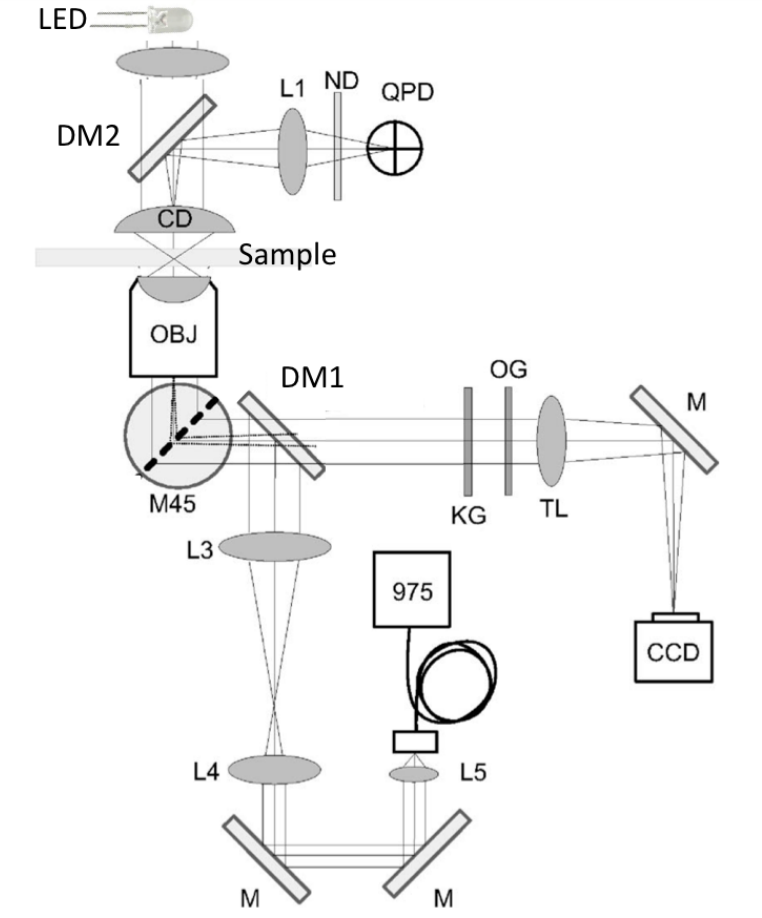
\includegraphics[width=0.7\textwidth]{Bilder/OP_Schema.png}
    \caption{Schematische Darstellung des Strahlengangs des Laserlichts durch den Aufbau der optischen Falle. Entnommen aus \cite{ref10}.}
    \label{fig:Aufbau}
\end{figure}
Dabei teilen sich die optische Pinzette und ein Mikroskop zum Beobachten der Probe 
zum Teil den Strahlengang. Das wird durch 
dichroitische Spiegel erreicht, die so arbeiten, dass sie  nur für das sichtbare Licht des
Mikroskops transparent sind und das Laserlicht im infraroten Bereich in den Strahlengang einkoppeln können.


Das Mikroskop arbeitet mit Licht im sichtbaren Bereich (Weißlicht-LED).
Dieses Licht wird über eine Linse und einen dichroitischen Spiegel fokussiert.
Über einen weiteren dichroitischen Spiegel fällt das Licht schließlich auf eine CCD Kamera.


Die optische Pinzette selbst arbeitet mit einem 975$\,$nm Laser.
Das Laserlicht wird über den gleichen dichroitischen Spiegel und ein 
Objektiv mit hoher numerischer Apertur auf die Probe fokussiert.
Detektiert wird das Signal mit einer Viersegment-Photodiode. 
Diese erlaubt neben der Bestimmung des Detektorsummensignals auch die Bestimmung der Auslenkung des Laserstrahls in x- und y-Richtung.

Die Probe befindet sich zwischen einer Kondensorlinse und einem Ölimmersionsobjektiv, bei dem ein 
Öltropfen verwendet wird um eine kontinuierlichere Änderung des Brechungsindex herbeizuführen und somit die numerische Apertur zu erhöhen.
Die Position der Probe kann mit Piezomotoren oder manuell über Mikrometerschrauben in allen drei Raumrichtungen eingestellt werden.

\subsection{Durchführung}
Zunächst soll eine Probe freier Quarzkügelchen in Wasser präpariert werden
und damit die Position der optischen Falle in den Aufnahmen der CCD-Kamera
bestimmt werden.

Mit einer Probe von fixierten Quarzkügelchen (NaCl-haltiges Wasser)
soll die Positionskalibrierung der Software in Abhängigkeit der 
Laserleistung durchgeführt werden. Die Konversionsfaktoren für die x- und y-Richtung lassen 
sich im Anschluss aus den Steigungen des linearen Bereichs der Kurven bestimmen. Außerdem soll das Diodensummensignal in Abhängigkeit des z-Piezo-Wertes 
aufgenommen werden, welches das axiale Positionssignal einer Kügelchen-Bewegung relativ zur Falle beschreibt.

Anschließend wird wieder mit freien Quarzkügelchen die Kraftkalibration der Software durchgeführt.
Zunächst ohne Krafteinwirkung in Abhängigkeit der Laserleistung und im Anschluss unter Einfluss einer oszillierenden Bewegung von außen.
Dabei soll hier in Abhängigkeit der Laserleistung untersucht werden, wann ein Kügelchen die Falle verlässt.
Abschließend soll der Einfluss eines Vortex-Retarders (ein 2$\pi$-Phasenmodulator) auf die Fallenkraft untersucht werden.

Der letzte Teil des Versuchs besteht aus dem Untersuchen von Vesikeln in Zwiebelzellen.
Dabei soll zunächst die Reaktion der Vesikel auf das Einfangen durch die optische Falle untersucht werden.
Anschließend wird der Durchmesser eines Vesikels durch Bildschirmaufnahmen bestimmt. 
Um die Geschwindigkeit zu ermitteln, wird durch die Photodiode gemessen, wie lange ein Vesikel das Laserlicht reduziert.
Zum Schluss soll untersucht werden, ab welcher Laserleistung der Aktin-Myosin-Motor die optische Falle nicht mehr überwinden kann.